\begin{abstract}
When payload-sway measurements arrive late, the crane's drive and cable-length measurements may already describe a newer state. We compare quadratic completion of the missing angle samples, direct forecasts from the last measured angle using six modal experts, and an age-weighted blend of the two. Model selection used one previously inspected Inteco record per motion family and ages up to 200~ms. Seven other previously inspected records were used for a retrospective stress test with imposed delays. At 100~ms age, mean absolute angular error without added jitter was 0.566\degs{} for the blend, 0.667\degs{} for completion and 0.626\degs{} for the direct bank. At 250~ms, outside the selection grid, the bank outperformed the blend on all seven records (0.692\degs{} versus 0.742\degs). At that age and a 100~ms forecast horizon, the direct bank scored 0.583\degs{}, the earlier autoregressive reference 0.666\degs{} and the blend 0.700\degs. The blend also inherits its zero-age forecast from an earlier synchronous estimator that already includes autoregressive components. These results characterize when blending helps on the archived records. Independent confirmation on newly acquired trials remains open.
\end{abstract}

\noindent\textbf{Keywords}\quad crane payload sway, sensor age, modal forecasting, cable length, autoregressive models

\section{Introduction}

A sway forecast has two relevant times when the angle arrives late. The latest received angle describes the payload at its acquisition time. The forecast describes the payload at a horizon after the current time, when trolley position, jib angle or cable length may already be available. Vision-based sway sensing motivates this distinction. Kaneko et al.~\cite{kaneko2009} report image-processing times on the order of tens to hundreds of milliseconds as a motivation and impose a 240~ms detection delay in their scaled-plant experiment. Tysse et al.~\cite{tysse2020} combine camera observations and an extended Kalman filter on a scaled knuckle-boom crane. The 0--250~ms range here is a synthetic stress grid of 0--25 samples at 100~Hz. The Inteco dataset provides a common acquisition grid, with no corresponding distribution of measured arrival times.

Delayed measurements have a long history in state estimation. Larsen et al.~\cite{larsen1998} study delayed observations in discrete-time Kalman filtering, including projection of a late measurement and correction of its gain. A chronological alternative for the known-age case is to assimilate angles at their acquisition times and propagate the estimated state forward using support measurements available through the current origin. We compare that approach with an estimator that completes the missing angle history and a bank that predicts directly from the dated history.

Earlier crane studies have used cable length and payload mass in data-driven predictors~\cite{kusznir2022}, physics-informed neural networks for travelling mobile cranes~\cite{zhou2025}, and learned prediction models in model predictive control~\cite{kusznir2024mpc,mao2026}. In related crane-control studies, Alhassan et al.~\cite{alhassan2024control} combine input shaping and fuzzy feedback, Talapiden et al.~\cite{talapiden2026control} combine neural adaptive input shaping and feedback under hoisting, and Shehu et al.~\cite{shehu2026control} study control with partial state measurements. Rehman et al.~\cite{rehman2022} adapt input shaping to cable length and payload mass. Their studies concern how to move the crane and suppress sway. Here the crane follows its recorded trajectory, and the output is a forecast of the encoder angle under the stated information available at each origin.

We estimate the incremental value of blending the two delay treatments by comparing it with both components, then use two archived autoregressive references to show how the ranking depends on the comparator and the record. An additional timestamp-aware estimator provides a conventional reference under the same input timing. The imposed ages and timestamp offsets probe a specific asynchronous measurement problem. Future work on hardware would need acquisition and arrival timestamps and would need to evaluate control performance separately.

\section{Data and forecast protocol}
\label{sec:protocol}

\subsection{Experimental platform and instrumentation}

The measurements were collected on an Inteco laboratory tower crane at Nazarbayev University~\cite{alhassan2025dataset,mendeley2025}. The rig measures $1.2\times1.2\times1.5$~m. Three DC motors actuate radial trolley travel $x$, jib rotation $J$ about the tower axis, and hoisting through the cable length $L$. The load can sway along two unactuated axes, measured as $\theta$ and $\beta$ at the suspension. The resulting system has five degrees of freedom and three drives. Figure~\ref{fig:inteco} shows the rig, its power interface, emergency stop and data-acquisition system.

\begin{figure}[H]
\centering
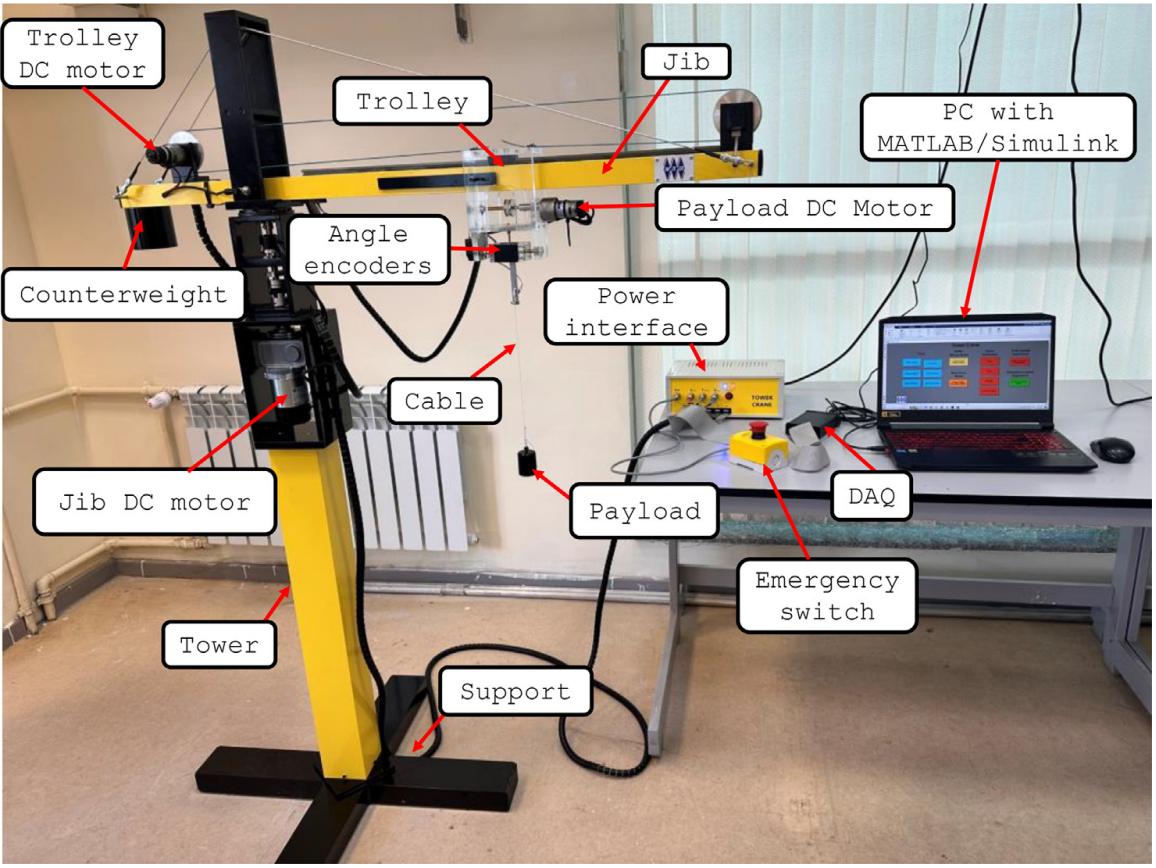
\includegraphics[width=.64\linewidth]{figures/inteco.png}
\caption{Inteco tower-crane apparatus used to collect the source dataset. The labelled photograph identifies the three drives, sway encoders and acquisition hardware. Reproduced from Alhassan et al.~\cite{alhassan2025dataset}, Fig.~2, under CC BY-NC 4.0.}
\label{fig:inteco}
\end{figure}

Three drive-mounted position encoders record trolley displacement, jib rotation and cable length. Two further encoders at the payload suspension measure the sway angles. The nominal angular increment of the sway encoders is one revolution divided by 4,096, or $0.0879$\degs{} ($0.001534$~rad). The source records angles in radians. We report angular errors in degrees. The physical positions and sway channels used in each motion family are listed in Table~\ref{tab:channels}.

\begin{table}[H]
\centering\small
\caption{Channels used by the benchmark. Trolley and jib refer to the actuated support motion, with or without hoisting. Reference units follow the dataset paper. The model reads the logged values directly.}
\label{tab:channels}
\begin{tabular}{@{}llllll@{}}
\toprule
Channel & Symbol & Unit used & Trolley & Jib & Combined \\
\midrule
Trolley displacement & $x$ & m & Yes & -- & Yes \\
Trolley reference & $x_r$ & m (source) & Yes & -- & Yes \\
Jib rotation & $J$ & rad & -- & Yes & Yes \\
Jib reference & $J_r$ & rad (source) & -- & Yes & Yes \\
Cable length & $L$ & m & Yes & Yes & Yes \\
Longitudinal sway & $\theta$ & rad & Yes & Yes & Yes \\
Transverse sway & $\beta$ & rad & -- & Yes & Yes \\
\bottomrule
\end{tabular}
\end{table}

\subsection{Recorded scenarios and preprocessing}

The data authors applied prescribed reference trajectories in open-loop experiments and logged the motion with MATLAB/Simulink R2022a. Each record contains 9,901 samples on the same 100~Hz grid from 0 to 99~s. The version~2 archive provides one spreadsheet per scenario and a separate common time spreadsheet. Our importer checks the file identities, finite values and the sample grid before forming forecast histories. The archived signals provide both the encoder histories and the later encoder angles used for scoring.

The standard payload is a 300~g solid cylinder. The remaining load types are a 75~g hollow ball, a 170~g hollow cylinder and a 500~g beam. For each family, the source contains fixed-length runs with the standard payload, plus hoisting or alternate-payload runs. The latter change more than one condition across the corpus, which limits attribution of an error difference to cable length alone. The earlier MATLAB study restricted the comparison to the 23 standard-payload, fixed-length runs. The present benchmark assigns all 33 records to fitting, validation or retrospective scoring. The 23 fitting records below are a different set from the 23 fixed-length records in the MATLAB study.

\begin{table}[H]
\centering\small
\caption{Scenario groups in the published dataset. Cable lengths are nominal experimental settings in metres. The dashes in the record columns indicate an absent combination.}
\label{tab:scenarios}
\begin{tabular}{@{}p{.32\linewidth}llccc@{}}
\toprule
Payload and length setting & Mass & Cable length & Trolley & Jib & Combined \\
\midrule
Standard cylinder, fixed & 300~g & 0.1--0.8$^{\rm a}$ & 1--8 & 14--20 & 24--31 \\
Standard cylinder, hoisting & 300~g & 0.1--0.5 & 9 & 21 & 32 \\
Hollow ball, fixed & 75~g & 0.5 & 10 & 22 & -- \\
Hollow cylinder, fixed & 170~g & 0.5 & 11 & 23 & -- \\
Beam, fixed & 500~g & 0.5 & 12 & -- & -- \\
Beam, hoisting & 500~g & 0.2--0.6 & 13 & -- & 33 \\
\bottomrule
\end{tabular}

\parbox{\linewidth}{\small\smallskip $^{\rm a}$ The jib-only fixed-length series ends at 0.7~m.}
\end{table}

\subsection{Record split}

Table~\ref{tab:splits} lists the 23 fitting, three validation and seven replay records. Trolley motion is scored on one sway axis, and the other two families on both axes. This yields five family--axis cases for model selection and 12 record--axis pairs for replay. The three validation records have the standard payload and fixed cable lengths. Each of the seven retrospective records has hoisting, an alternate payload, or both. They are a stress test under shifted operating conditions. All 33 records were inspected during earlier development. The seven retrospective records were excluded from fitting and selection in this experiment, but the comparison is not an independent test.

\begin{table}[htbp]
\centering
\caption{Inteco record IDs and sway axes in the dated-angle experiment.}
\label{tab:splits}
\begin{tabular}{@{}lllll@{}}
\toprule
Motion family & Axes & Fit & Validation & Replay \\
\midrule
Trolley & $\theta$ & 1, 2, 3, 5--8, 10--12 & 4 & 9, 13 \\
Jib rotation & $\theta,\beta$ & 14--16, 18--20 & 17 & 21--23 \\
Simultaneous & $\theta,\beta$ & 24--27, 29--31 & 28 & 32, 33 \\
\bottomrule
\end{tabular}
\end{table}

\subsection{Available measurements and targets}

At forecast origin $t$, the latest angle sample was acquired at $t-a$, where $a$ is a known integer multiple of 10~ms. The models receive 401 angle samples ending at $t-a$ and 401 samples of cable length, support position and native drive-reference channels ending at $t$. Each history spans 4~s. The support channels are trolley position $x$, jib angle $J$, or both. The dataset paper labels $x_r$ in metres and $J_r$ in radians~\cite{alhassan2025dataset}. The models use the exported values without conversion to forces or accelerations. For example, in record~4 the logged $x_r$ spans 0.215--1.000 in the source units, while the measured $x$ spans 0--0.503~m. That difference does not identify a servo conversion. Independent data intake therefore checks the reference semantics and scale against the original export.

The targets are recorded angles at $t+h$ for $h\in\{0.10,0.20,0.35,0.50,0.75,1.00,1.50\}$~s. Thus the 100~ms target at an angle age of 250~ms lies 350~ms after the last measured angle. Future measured support motion, cable length and sway are excluded from the inputs. Validation and replay origins start at 4.25~s and advance in 1~s steps, preserving the full history at every age without padding the start of a record.

Age and noise are imposed on stored inputs. Validation uses ages of 0, 20, 50, 100, 150 and 200~ms. Replay adds ages of 30, 70 and 250~ms. Each setting uses either the recorded angle history or that history plus seeded uniform jitter of up to one encoder increment in either direction. The recorded target angles and support channels are shared across methods. The condition without added noise retains the original encoder quantization.

\begin{figure}[H]
\centering
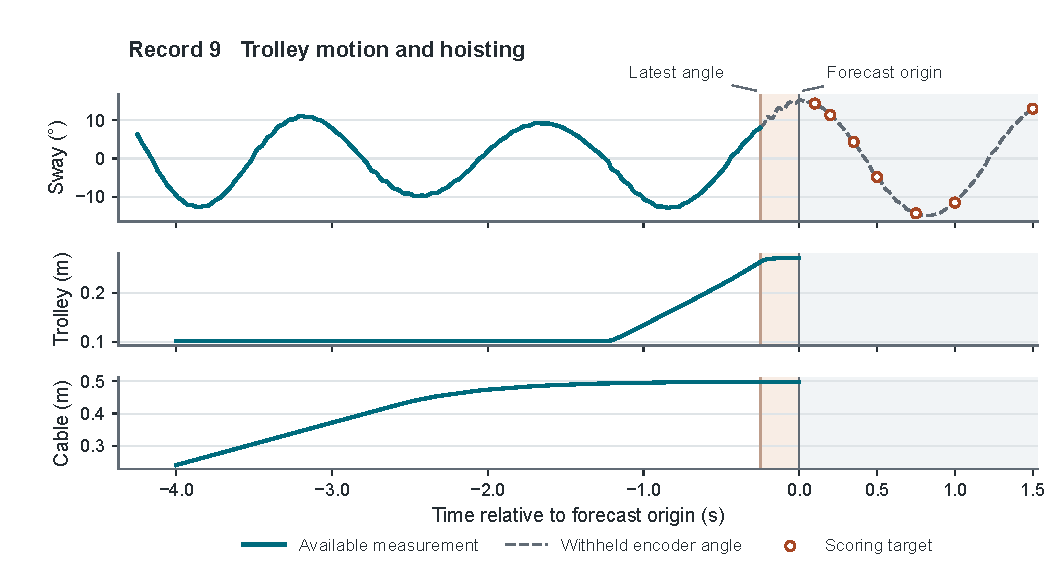
\includegraphics[width=.96\linewidth]{figures/dated_input_example.pdf}
\caption{Measured inputs and scoring targets for an illustrative 250~ms angle age on record~9 (trolley motion with hoisting), at the replay origin 5.25~s. The 401 sway samples end at 5.00~s, while the trolley and cable histories end at the origin. The dashed encoder trace is withheld from inference. Circles mark the seven scoring targets. The logged drive reference is omitted from the figure.}
\label{fig:dated-input}
\end{figure}

\section{Development and selection}
\label{sec:development}

The initial MATLAB study compared short-horizon angle-only predictors on fixed-length records. In the first Python experiments, a calibrated oscillator was competitive at longer horizons, and adding learned forcing helped some operating conditions while worsening others. Later work fitted oscillation modes to the recent angle history and combined them with autoregressive forecasts. A change that improved active-motion forecasts could also worsen forecasts during settled motion, which motivated the existing synchronous estimator's low-motion rule. The present study starts from that estimator and isolates the next decision: how to use a dated angle history. Appendix~\ref{app:development} preserves the earlier comparisons and their different protocols.

The known-age development study selected quadratic completion from eight ways to handle the missing angle samples. The subsequent dated-angle study evaluated 21 candidates at 0, 20, 50, 100, 150 and 200~ms, giving the five family--axis cases and both jitter settings equal weight. A single blend timescale was selected. The gate required at least a 3\% improvement over completion and at least 5\% over the earlier ARX, a win over that ARX in at least four of five cases, and at most 5\% higher error than completion at any validation age. The 100~ms blend passed all four checks. The separate dense ARX reference was selected later, with the blend held fixed. At 250~ms the blend's weight is extrapolated beyond the validation ages.

\section{Forecast methods}

\subsection{Completing the angle history}

The first component fits a quadratic to the last 0.25~s of available angle history. It extrapolates over the missing interval and passes the completed history to a previously fitted forecaster. That forecaster combines autoregressive and modal forecasts using recent support motion and forecast errors on already observed angles. The range of support motion over the past 4~s identifies low-motion packets, using thresholds of 2~mm for trolley position and 2~mrad for jib angle. In these packets the component retains its previous low-motion rule. We also report this component separately as quadratic completion.

\subsection{Forecasting from the dated angle}

The second component uses six modal experts. They fit a constant offset and oscillatory modes to the last 2.5~s of observed angle history, sampled every 50~ms for the fit. The frequency search is scaled by the nominal frequency $\sqrt{g/\ell_{\rm eff}}$, with a positive effective length $\ell_{\rm eff}$ calibrated on fitting records. Four experts align past support measurements to the angle history and use measured support motion through the sensor gap. Beyond $t$ they assume either held or linearly continued support position. Each continuation has one expert with fixed coupling and one with a local regularized update of the fitted coupling. The other two experts describe free motion, one with constant length and one with measured length through the gap followed by held length. Table~\ref{tab:experts} lists the six alternatives. Appendix~\ref{app:forcing} defines the forcing basis and how its coefficients are fitted.

\begin{table}[H]
\centering\small
\caption{Forecasts in the direct bank. The four forced experts use measured support motion across the gap between the last angle measurement and the origin. Future support and length shown here are model assumptions.}
\label{tab:experts}
\begin{tabular}{@{}llll@{}}
\toprule
Expert & Forcing coupling & Future support & Length treatment \\
\midrule
Constant-length free & -- & -- & Constant \\
Held support, fixed & Fitted on training records & Hold position & Constant \\
Held support, adapted & Local update & Hold position & Constant \\
Linear support, fixed & Fitted on training records & Linear extrapolation & Constant \\
Linear support, adapted & Local update & Linear extrapolation & Constant \\
Changing-length free & -- & -- & Measured gap, then held \\
\bottomrule
\end{tabular}
\end{table}

In the changing-length expert, a modal coordinate $z_j$ follows the local approximation
\begin{equation}
 \ddot z_j(s)+\left(d_j+2\frac{\dot\ell(s)}{\ell(s)}\right)\dot z_j(s)
 +\kappa_j\frac{\ell(t-a)}{\ell(s)}z_j(s)=0 ,
 \label{eq:variable-length}
\end{equation}
where $d_j$ and $\kappa_j$ are modal damping and stiffness at measurement time, and $\ell(s)$ is the calibrated effective length evaluated from the logged $L(s)$, held at $\ell(t)$ beyond the origin. The length-rate term follows the small-angle variable-length pendulum equation~\cite{belyakov2009,gonzalez2017}. The empirical modes approximate sway along one measured axis at a time.

The bank assigns weights using six forecasts from a history with origin $t-1$~s. The horizons relative to that origin are $0.10$, $0.20$, $0.35$, $0.50$, $0.70$ and $1-a$~s, where $a$ is expressed in seconds. All six angle targets are available by $t$, with the last at $t-a$. The earlier packet uses its own assumed continuation of support motion. Let $E$ contain its six prediction errors for each expert and $w_0$ be the prior weights. The bank solves
\begin{equation}
 \min_w \frac{1}{6}\lVert Ew\rVert_2^2+\lambda\lVert w-w_0\rVert_2^2,
 \qquad w_j\ge 0,\quad \sum_{j=1}^{6}w_j=1 ,
\end{equation}
where $\lambda=\lVert E\rVert_F^2/36+q^2/12$ and $q$ is the encoder increment in the angle units used for fitting. The prior assigns half the weight to each of the two free-motion experts in low support motion. In higher support motion each free expert receives a quarter and each forced expert receives an eighth. The fitted weights then apply to all seven current forecast horizons, including 1.50~s.

\subsection{Age-weighted blend and ARX references}

The blend uses
\begin{equation}
 \widehat\theta(t+h)=(1-\alpha)\widehat\theta_{\rm completion}(t+h)
                    +\alpha\widehat\theta_{\rm bank}(t+h),
 \qquad \alpha=\frac{a}{a+100\,\mathrm{ms}} .
 \label{eq:mixture}
\end{equation}
At age zero, the implementation bypasses the bank and returns the synchronous estimator for the blend, completion and the bank column. The synchronous estimator already combines autoregressive and modal forecasts. Internal validation selected this mixture from 21 candidates, including standalone modal forecasts, alternative bank regularization and other blends. The selection, identified as \texttt{mix\_bank\_10} in the repository, was fixed before replay.

The dense ARX reference includes angle-only and input--output feature sets, length-dependent coefficients, direct forecasts and corrections to modal forecasts. Its pool retains 3~s and 4~s history variants and alternative ways to handle missing angle samples. The expanded pool includes 120 new fits and offers 304 options per family--axis case, including some identical predictions. The original dense fits and the new age-augmented fits use 0.25~s steps between training origins. The pipelines have comparable access to fitting records, channels and dense origin support. Their transformations and objectives differ.

We retain the earlier ARX as the main archived autoregressive comparison because it performs better than dense ARX at positive ages from 50~ms onward in the retrospective sample. This choice of presentation follows inspection of the errors. Both ARX variants had already been fixed using validation. They select a configuration for each family--axis case and each of six validation ages. For 30, 70 and 250~ms they use the configuration selected at 20, 50 and 200~ms, respectively. Both still receive the supplied exact age for timestamp alignment or age-aware features as appropriate. The blend uses the supplied age in its weight rule as well. The bank fits modes within each history, whereas the archived ARX coefficients are fitted on the training records.

\subsection{Additional delayed-measurement references}
\label{sec:added-baselines}

After the original replay was inspected, we added a timestamp-aware Kalman reference, a local autoregression and three simple references. They use the original fitting and validation roles, origins, horizons and jitter realizations. A preliminary Kalman run used the injected jitter variance. For the final comparison we fixed the observation variance at $q^2/12$ in both conditions, selected settings on the three validation records, and froze those settings before rerunning the seven-record comparison. This comparison is post hoc at the study level.

The Kalman filter uses a linear time-varying small-angle oscillator for each axis. Let $\delta$ be sway about a local equilibrium, $v=\dot\delta$, and $b$ be an encoder-angle offset that follows a random walk. The measurement is $\theta=\delta+b+\epsilon$. The drift equations are
\begin{equation}
 \dot \delta=v,\qquad
 \dot v=-\frac{g}{\ell_{\rm eff}(s)}\delta
 -\left[d+\operatorname{clip}\!\left(2\dot\ell_{\rm eff}/\ell_{\rm eff},-2,2\right)\right]v+u(s).
\end{equation}
The effective length is calibrated on fixed-length training segments. The drive term $u$ is fitted on the training records by regressing an angular-acceleration residual on measured support acceleration and applicable rotation terms. At forecast time, backward quadratic fits over 0.20~s supply support derivatives. Process noise represents uncertain acceleration and a slowly changing offset. The measurement variance is fixed at $q^2/12$ in both jitter conditions.

Angle updates stop at the acquisition time $t-a$. The state then propagates to $t$ using the available support and length measurements. For angle samples predating the oldest support sample, the filter holds the earliest measured length and sets the forcing and length rate to zero. After $t$ it holds length fixed and uses either zero forcing or the latest estimated forcing decayed with a 100~ms time constant. The validation grid for each case contains 18 combinations of damping, process noise scale and forcing continuation. The filter assimilates the measurements in acquisition order and rolls the estimate through the known gap. It implements the benchmark's ordered, uniform-age observation pattern.

The local AR fits a centred ridge autoregression to the same 2.5~s angle span sampled every 50~ms as the direct bank. The order (four or eight lags) and ridge strength are selected on validation. The fit at each origin uses only the available angle history. Unstable fitted poles are contracted, and interpolation evaluates the recursive forecast at $a+h$. The calibrated oscillator fits an offset and one sinusoidal mode over the same span, with its frequency set by the training calibration at the last available angle. Persistence repeats that last angle and the zero reference always predicts zero.

\subsection{Selection score and retained comparisons}

For each family--axis case, angle age and noise level, we average the absolute error over origins and horizons separately for low and high recent support motion, then give the two groups equal weight. Low support motion can include hoisting. The overall selection score gives equal weight to the five cases, six ages and two noise levels. This avoids choosing primarily on the more numerous low-motion origins. The all-origin replay average in Sec.~\ref{sec:results} answers a different question.

Figure~\ref{fig:validation-selection} shows the comparison that determined the blend and the reference challenge that followed. The 100~ms blend reduced the development MAE by 14.7\% relative to quadratic completion and 12.2\% relative to earlier ARX, using the unrounded scores. At zero age, completion and the blend coincide by design. The greatest separation between them on this validation grid occurs at 200~ms. Among the individual experts, the lowest validation score came from the fixed-coupling model with linear support continuation. Its validation score was 1.804\degs{} compared with 1.833\degs{} for the regularized direct bank. Among these candidates the blend had the lowest validation error.

\begin{figure}[H]
\centering
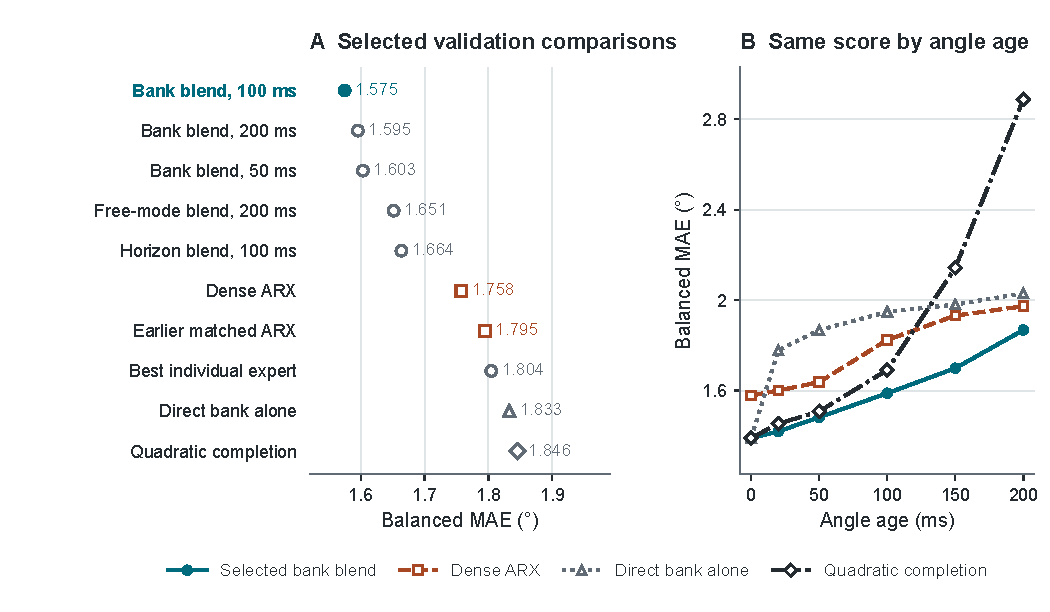
\includegraphics[width=.96\linewidth]{figures/dated_validation_selection.pdf}
\caption{Validation comparisons preceding the seven-record replay. Panel A shows representative candidates from the 21-variant search, together with the ARX references. The times in the blend labels are the offsets in the denominator of the age weight. Panel B averages balanced MAE at each age across five cases and both noise levels. Dense ARX was fitted after selection of the blend.}
\label{fig:validation-selection}
\end{figure}

\begin{table}[H]
\centering\small
\caption{Balanced validation MAE by family and axis, in degrees. Both ARX references are evaluated on the same validation grid as the blend. The bottom row weights the five cases equally.}
\label{tab:validation-cases}
\begin{tabular}{@{}lrrr@{}}
\toprule
Case & Blend & Dense ARX & Earlier ARX \\
\midrule
Trolley, $\theta$ & 0.582 & 0.619 & 0.621 \\
Jib, $\theta$ & 1.269 & 1.625 & 1.642 \\
Jib, $\beta$ & 1.402 & 1.554 & 1.620 \\
Combined, $\theta$ & 2.399 & 2.446 & 2.446 \\
Combined, $\beta$ & 2.221 & 2.545 & 2.644 \\
\midrule
Mean & 1.575 & 1.758 & 1.795 \\
\bottomrule
\end{tabular}
\end{table}

\section{Results}
\label{sec:results}

\subsection{What blending adds}
\label{sec:incremental}

We score mean absolute error (MAE) against the measured encoder angle. The retrospective mean averages origins and horizons within each axis, axes within each physical record, and then the seven records equally. The two jitter conditions share the same targets. Table~\ref{tab:age-mae} reports the unperturbed-history condition. The full tables retain both conditions and all records and horizons.

\begin{table}[H]
\centering\small
\caption{Retrospective MAE by imposed angle age, in degrees, without added jitter. At 0~ms all three delay treatments return the same synchronous estimator. The bank is evaluated separately at positive ages. The 250~ms row is outside the validation grid.}
\label{tab:age-mae}
\begin{tabular}{@{}rrrrrr@{}}
\toprule
Age (ms) & Blend & Completion & Direct bank & Earlier ARX & Dense ARX \\
\midrule
0 & 0.525 & 0.525 & 0.525 & 1.074 & 1.071 \\
20 & 0.531 & 0.555 & 0.607 & 1.096 & 1.076 \\
30 & 0.530 & 0.560 & 0.610 & 1.115 & 1.084 \\
50 & 0.535 & 0.577 & 0.618 & 1.061 & 1.145 \\
70 & 0.545 & 0.606 & 0.615 & 1.094 & 1.170 \\
100 & 0.566 & 0.667 & 0.626 & 1.077 & 1.183 \\
150 & 0.604 & 0.846 & 0.635 & 1.076 & 1.159 \\
200 & 0.669 & 1.110 & 0.665 & 1.232 & 1.307 \\
250 & 0.742 & 1.479 & 0.692 & 1.246 & 1.316 \\
\bottomrule
\end{tabular}
\end{table}

The inherited synchronous estimator scores 0.525\degs{} at zero age, against 1.071\degs{} for dense ARX and 1.074\degs{} for earlier ARX. Its gap of about 51\% versus dense ARX precedes the delay treatment. The earlier-ARX gap is 0.549\degs{} at zero age and 0.503\degs{} at 250~ms. Figure~\ref{fig:delay-compensation} compares the blend with its two components. At 100~ms, the blend lowers mean MAE by 0.101\degs{} against completion and by 0.060\degs{} against the direct bank. At 200~ms the bank has slightly lower mean error than the blend. At 250~ms it improves on the blend by 0.050\degs{} and does so in every physical record.

\begin{figure}[H]
\centering
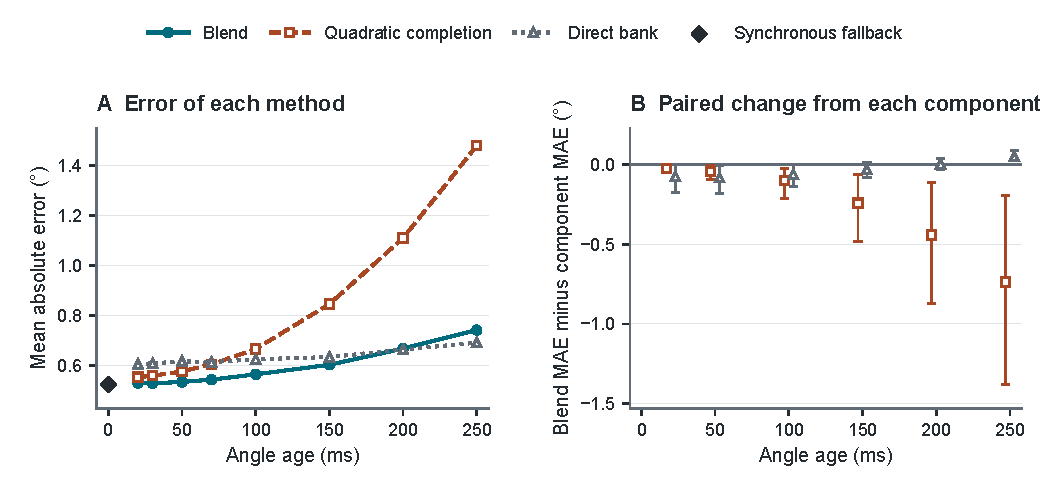
\includegraphics[width=.96\linewidth]{figures/delay_compensation.pdf}
\caption{Incremental comparisons on seven previously inspected records without added jitter. Panel A gives the equal-record mean MAE. The zero-age diamond is the synchronous fallback. Panel B shows paired blend-minus-component differences. Negative values favour the blend. Bars show descriptive 95\% percentile intervals from 20,000 paired resamples of the seven whole records.}
\label{fig:delay-compensation}
\end{figure}

Table~\ref{tab:paired} adds the median paired difference and the number of records favouring the blend. The bootstrap resamples whole records with replacement, using the same draws for each pair. These intervals describe this small retrospective sample. Windows, axes, ages and horizons within a record are not counted as independent trials.

\begin{table}[H]
\centering\small
\caption{Paired blend-minus-reference MAE in degrees at 100 and 250~ms, without added jitter. Negative values favour the blend. Intervals are descriptive 95\% percentile intervals for the paired mean.}
\label{tab:paired}
\begin{tabular}{@{}rlrrlr@{}}
\toprule
Age (ms) & Reference & Mean & Median & Interval & Blend wins \\
\midrule
100 & Completion & $-0.101$ & $-0.046$ & $[-0.214, -0.023]$ & 6/7 \\
100 & Direct bank & $-0.060$ & $-0.042$ & $[-0.137, +0.002]$ & 4/7 \\
100 & Earlier ARX & $-0.511$ & $-0.136$ & $[-0.934, -0.159]$ & 7/7 \\
100 & Dense ARX & $-0.617$ & $-0.764$ & $[-0.959, -0.295]$ & 7/7 \\
250 & Completion & $-0.736$ & $-0.257$ & $[-1.380, -0.192]$ & 7/7 \\
250 & Direct bank & $+0.050$ & $+0.041$ & $[+0.023, +0.088]$ & 0/7 \\
250 & Earlier ARX & $-0.503$ & $+0.011$ & $[-1.102, +0.019]$ & 3/7 \\
250 & Dense ARX & $-0.574$ & $-0.172$ & $[-1.096, -0.145]$ & 5/7 \\
\bottomrule
\end{tabular}
\end{table}

\subsection{Short-horizon loss at the longest age}

The 250~ms age and 100~ms horizon cell separates the bank's performance from the blend's. Without added jitter, completion scores 1.733\degs{} and the bank scores 0.583\degs. The blend scores 0.700\degs, above both archived ARX references. The bank has lower error than either ARX in that cell under both jitter settings (Table~\ref{tab:short-cell}). At 250~ms, the bank has lower mean error than the blend at five of seven horizons, and lower seven-horizon error in all seven records. In the short-horizon cell, dense ARX has lower MAE than the blend on six records by numerical sign, including a gap below 0.005\degs{} on record~32 under both jitter settings. This gap is small relative to the encoder increment.

\begin{table}[H]
\centering\small
\caption{MAE in the 250~ms age and 100~ms horizon cell, in degrees. Added jitter is uniform on the indicated interval and is applied only to the input angles.}
\label{tab:short-cell}
\begin{tabular}{@{}lrrrrr@{}}
\toprule
Added jitter & Blend & Completion & Direct bank & Earlier ARX & Dense ARX \\
\midrule
None & 0.700 & 1.733 & 0.583 & 0.666 & 0.653 \\
$\pm 1$ increment & 0.702 & 1.738 & 0.587 & 0.675 & 0.660 \\
\bottomrule
\end{tabular}
\end{table}

\subsection{Dependence on the ARX reference and record}

Dense ARX scored better in internal validation than earlier ARX (1.758\degs{} versus 1.795\degs). On the retrospective records, earlier ARX has lower all-origin MAE at every sampled age from 50 to 250~ms. At 250~ms the blend's mean is 0.503\degs{} below earlier ARX, while the median paired difference is 0.011\degs{} above it and the blend wins on three of seven records. The corresponding count against dense ARX is five of seven.

\begin{figure}[H]
\centering
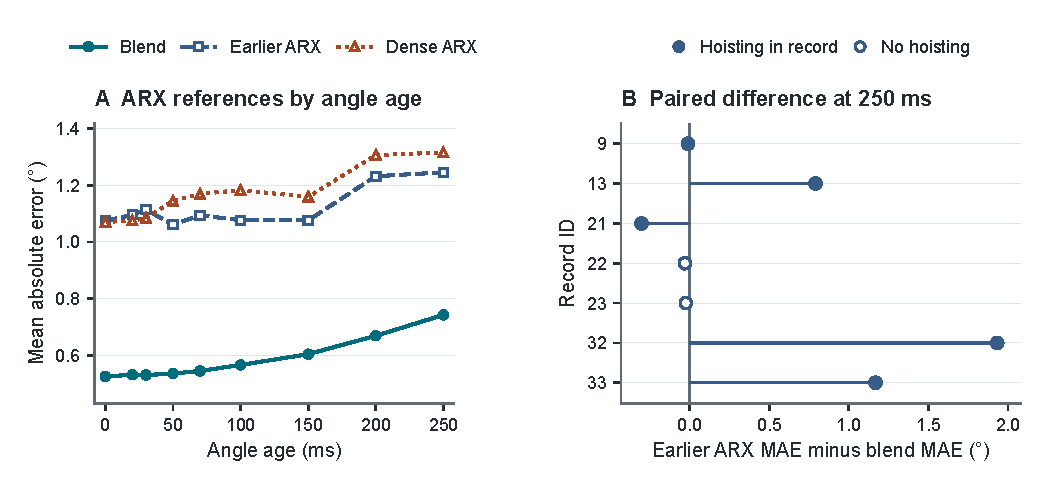
\includegraphics[width=.96\linewidth]{figures/arx_reference_replay.pdf}
\caption{Comparison with both frozen ARX references, without added jitter. Panel A averages seven horizons and seven records equally. Panel B shows earlier ARX minus blend MAE at 250~ms by physical record. Positive values favour the blend. Filled markers identify records with hoisting.}
\label{fig:arx-retrospective}
\end{figure}

Records 13, 32 and 33, which all include hoisting, account for 110\% of the net mean reduction against earlier ARX at 250~ms. The blend is worse by 0.092\degs{} on average on the remaining four records. The mean reduction is 0.716\degs{} across the five hoisting records. Across the two records without hoisting, both jib rotations with alternate loads, the blend is worse by 0.027\degs. These comparisons by record type combine differences in motion, payload and excitation. Appendix~\ref{app:record-gaps} gives the differences at every age.

\subsection{Results for the additional delayed-measurement references}
\label{sec:additional-results}

Table~\ref{tab:added-baselines} gives the scores for the post-hoc references on the same seven retrospective records. A parity check matched all 216 record--axis--age--jitter packets to the archived origin indices and recomputed the archived dense-ARX MAE from the same target indices. The maximum absolute discrepancy was below $7\times10^{-15}$~degrees. The Kalman reference scored 1.795\degs{} on balanced validation, and local AR scored 2.441\degs. With no added jitter, the Kalman reference scored 1.134\degs{} at 100~ms and 1.325\degs{} at 250~ms across horizons. At 250~ms and the 100~ms horizon it scored 1.055\degs{} without jitter and 1.068\degs{} with jitter, compared with 0.583\degs{} and 0.587\degs{} for the direct bank, respectively. This evaluates one fitted, separate-axis small-angle state model. A coupled or nonlinear filter, or a filter tuned on new acquisitions, could give a different result.

\begin{table}[H]
\centering\small
\caption{Additional reference MAE in degrees, without added jitter. The first three columns average the seven forecast horizons. The last column evaluates the 100~ms horizon at 250~ms age. Each column gives physical records equal weight.}
\label{tab:added-baselines}
\begin{tabular}{@{}lrrrr@{}}
\toprule
Reference & 100~ms & 200~ms & 250~ms & 250~ms, short horizon \\
\midrule
Timestamp-aware Kalman & 1.134 & 1.245 & 1.325 & 1.055 \\
Local AR & 1.662 & 1.792 & 1.864 & 1.453 \\
Calibrated oscillator & 2.112 & 2.205 & 2.249 & 1.844 \\
Persistence & 8.151 & 8.833 & 9.148 & 7.497 \\
Zero forecast & 7.445 & 7.445 & 7.445 & 7.488 \\
\bottomrule
\end{tabular}
\end{table}

\subsection{Sensitivity to the reported measurement age}

An archived experiment without added jitter changes the reported age while leaving histories and targets fixed. The true ages are 0, 20, 50, 100, 150, 200 and 250~ms. The offsets $-20$, $-10$, 0, $+10$ and $+20$~ms give 31 admissible combinations within the supported range. The same five interior ages support all offsets. For these ages, overstating by 10~ms adds 0.112\degs{} to blend MAE and 0.121\degs{} to dense ARX MAE. At $+20$~ms the absolute increases are similar, 0.288\degs{} and 0.300\degs, with relative increases of 49.5\% and 25.6\% from different starting errors. Understating by 20~ms increases blend MAE by 0.202\degs{} and reduces dense ARX MAE by 0.011\degs{} on this grid.

\begin{figure}[H]
\centering
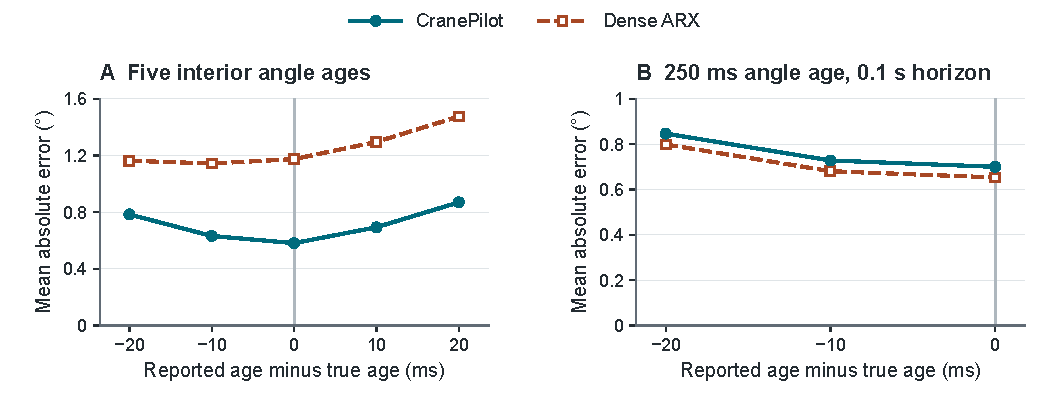
\includegraphics[width=.96\linewidth]{figures/timestamp_sensitivity.pdf}
\caption{Sensitivity of the archived blend and dense ARX to the supplied angle age. A positive offset overstates age. Panel A uses the same five true ages at every offset. Panel B uses 250~ms true age and 100~ms horizon, for which positive offsets fall outside the supported range. The CranePilot curve denotes the blend.}
\label{fig:timing}
\end{figure}

\section{Discussion}

At 100~ms, the blend reduced the mean error relative to both components, though its advantage over the direct bank varied across records. At 200~ms the two mean errors were close. At 250~ms, the bank performed better on every record. The blend still assigns completion $100/(250+100)\simeq29\%$ weight at that age. Removing completion from this archived comparison eliminates the 100~ms-horizon loss against both ARX references. This observation motivates a comparison of bank-only and blend forecasts at long ages on new data. The current comparison leaves the selected rule fixed.

For an ideal small-angle pendulum, $T=2\pi\sqrt{L/g}$. A 250~ms gap spans about $142^\circ$ of phase for a 0.1~m rope and $63^\circ$ for a 0.5~m rope. Quadratic completion extrapolates a 250~ms fitting window over another 250~ms at this setting. A long extrapolation relative to the period can distort the completed angle history. These nominal phase values illustrate the scale of the gap. The fitted modal periods and dynamics can differ, particularly under hoisting or for a distributed payload.

The evidence is limited by its experimental units. The five validation cases share three recordings, and the seven stress-test records come from the same rig. Resampling the seven paired records describes variation in this sample. It cannot account for repeated decisions across earlier development or provide a population-level estimate of generalization. Trolley, jib and combined motions also differ in the amount of active support motion, payload and changing length. Separate-axis models omit explicit coupling between the two sway states as the jib rotates. The archived study uses encoder angles as targets and leaves all recorded crane trajectories unchanged during the imposed timing perturbations.

In an earlier transfer experiment on four camera records from another rotary crane~\cite{khemakhem2026}, an older CranePilot model scored 0.895\degs{} MAE, compared with 0.376\degs{} for persistence, 0.266\degs{} for a geometric reference and 0.038\degs{} for a locally fitted ARX residual. That experiment used a different sensing rate and information set. It provides a concrete reason to include local baselines and limits claims about transfer of the older model.

\subsection{Independent confirmation}

The existing prospective protocol freezes the blend and dense ARX, along with the information available at each origin, the grouping of physical trials and the primary score. It calls for at least five declared conditions and five independent acquisition clusters. The score weights conditions, trials within conditions, axes within trials, and horizons and origins within axes. Its success criteria are at least 10\% lower MAE, a strict majority of condition wins and an upper 97.5th percentile below zero for a paired difference resampled by physical cluster. These thresholds apply to the existing protocol. Including the bank, earlier ARX and the added estimators as prospective comparators would require a dated amendment before seeing new outcomes. Same-rig trials from new acquisition sessions would allow an independent evaluation. Actual delay testing also requires acquisition and arrival timestamps for the angle and evidence that support measurements are current at the forecast origin. Suitable new trials have yet to be received.

\section{Conclusion}

On the retrospective Inteco stress test, combining quadratic completion and direct modal forecasting improved mean MAE over either component at 100~ms angle age. At 250~ms, outside the validation grid, the direct bank gave lower error than the blend on all seven records and recovered the short-horizon comparison against both archived ARX references. At zero age the blend inherits its forecast from the synchronous estimator, so its zero-age advantage over ARX does not measure the contribution of delay handling. These comparisons delimit the conditions in which the blend is useful on the archived records. Independent physical trials are needed to establish whether the same pattern transfers.

\section*{Data and code availability}

The Inteco dataset is available at \url{https://doi.org/10.17632/x69hyyv3zw.2}~\cite{mendeley2025}. The source, frozen model choices, figure scripts and record-level tables are available in the repository.
\begin{quote}\url{https://github.com/kutyrevratmir3-design/cranepilot}\end{quote}
The original replay is tied to snapshot \texttt{f3107fe}. The paired reanalysis and additional baselines use the same archived records. The apparatus photograph is credited separately in Fig.~\ref{fig:inteco}.

\section*{Acknowledgments and disclosure}

The author thanks the creators of the Inteco dataset for making the measurements available. AI tools assisted in writing and reviewing research code, checking numerical results, generating plots and drafting and revising the manuscript.

\appendix
\section{Earlier forecasting experiments}
\label{app:development}

The forecasting task changed in three steps. The initial benchmark asked how far recent sway angles and cable length could predict motion on a new fixed-length record. A second benchmark supplied a planned drive command and examined whether a learned forcing correction improved the physical model. The final benchmark uses a longer measurement history, works without a supplied future command plan, and gives the models the age of the last angle sample. Table~\ref{tab:development-comparisons} records comparisons within these protocols. The fitting records, available inputs, scored origins and aggregation changed between stages.

\subsection{From one-step prediction to command-conditioned rollout}

The original MATLAB study evaluated fixed-length runs from the trolley, jib and simultaneous-motion families. It compared zero and persistence forecasts, linear regression, boosted trees and an ensemble of feed-forward networks. The learned models used three angle lags and cable length. On trolley record~1, linear regression gave a one-step mean absolute error (MAE) of $0.0796^\circ$ at 10~ms, near the $0.0879^\circ$ encoder increment. The one-step result motivated longer forecast horizons, where a small error in the fitted oscillation frequency can accumulate into a visible phase error.

The first Python benchmark trained on trolley records 3, 5 and 6, used record~4 for validation, and evaluated records 1, 2, 7 and 8. The evaluation lengths fell below and above the training range. A calibrated oscillator set the frequency from an effective length fitted on the training records. Training penalized components of a neural correction that aligned with the oscillator forecast sensitivities to frequency and damping. The projected residual helped at 100~ms and lost to the calibrated oscillator at 1~s. The plain oscillator therefore remained a reference at longer horizons.

The next benchmark added recent trolley position and native reference, a 41-sample history at 100~Hz, and the prescribed future reference. A separately fitted and frozen drive model produced the trolley acceleration for a forced oscillator. The phase-exact passive-memory predictor added four latent states and bounded the increase in storage by the work done by the supplied forcing. Its same-information Gaussian-process (GP) residual reference performed better at several short and intermediate horizons. Repeating the fit with matched training also reduced the error of the passive model itself. This made the matched-training model a closer comparator for a new observer and recurrent forcing correction than the original training run.

A later comparison selected a forced observer with a robust loss and a learned forcing correction. This model retained the best validation result on the primary split in the subsequent temporal-model campaign. On long-cable extrapolation the validation-selected temporal model reduced average MAE from $0.513^\circ$ to $0.497^\circ$, while active-origin MAE increased from $0.932^\circ$ to $0.968^\circ$. On short-cable extrapolation the selected alternative increased average MAE from $0.432^\circ$ to $0.439^\circ$. The primary driven model was therefore retained for that benchmark. The later history-only predictor uses a different input contract and does not require the fitted actuator or the planned command sequence.

\begin{table}[tbp]
\centering
\small
\caption{Selected paired comparisons from the development sequence. MAE is in degrees. Each row uses a common score and evaluation population for the two methods in that row. The table combines several distinct tasks.}
\label{tab:development-comparisons}
\renewcommand{\arraystretch}{1.14}
\begin{tabular}{@{}p{.34\linewidth}p{.39\linewidth}rr@{}}
\toprule
\raggedright Protocol and score & \raggedright Reference / candidate & Ref. & Cand. \\
\midrule
\raggedright Fixed length, 100~ms replay & \raggedright Calibrated oscillator / projected residual & 0.300 & 0.219 \\
\raggedright Fixed length, 1~s replay & \raggedright Calibrated oscillator / projected residual & 0.758 & 0.907 \\
\addlinespace[3pt]
\raggedright Planned-command replay, seven horizons & \raggedright Matched-training passive model / driven innovation & 0.524 & 0.512 \\
\raggedright Settled-input replay, seven records & \raggedright Strengthened ARX / local two-mode fit & 0.492 & 0.261 \\
\raggedright Active-motion validation, balanced score & \raggedright Matched ARX / drive-conditioned blend & 1.587 & 1.397 \\
\raggedright Synchronous replay, all origins & \raggedright Earlier soft blend / guarded fusion & 0.545 & 0.504 \\
\addlinespace[3pt]
\raggedright Known-age validation, ages 0--100~ms & \raggedright Angle hold / quadratic completion & 2.257 & 1.511 \\
\raggedright Dated-angle validation, ages 0--200~ms & \raggedright Quadratic completion / selected mixture & 1.846 & 1.575 \\
\bottomrule
\end{tabular}
\end{table}

\subsection{Local modal fits and the move to guarded fusion}

The next experiment asked whether the oscillation frequency could be estimated locally instead of extrapolating a calibration from training records. For residual sway with settled drive and cable length, it used four seconds of recent history, sampled for fitting every 50~ms. A fixed-frequency oscillator was compared with damped one- and two-mode fits. The frequency search used the training-calibrated frequency as a scale, and amplitudes and offsets were fitted to the available angles. Validation chose the two-mode option for all five family--axis cases. The candidate had lower mean MAE than a strengthened autoregressive reference on six of seven replay records. It lost on record~21, and the descriptive paired interval from resampling whole records included zero.

To use past prediction errors as a local measure of reliability, an early blend asked the modal model and ARX to forecast six angles within the final second of the available history. It then used their errors on those already observed angles to weight the new forecast. Replaying this blend outside the settled-input scope exposed a dependence on the operating regime. The modal model alone gave $2.351^\circ$ MAE in drive-only windows versus $1.805^\circ$ for the ARX reference. In low past motion the same models gave $0.266^\circ$ and $0.495^\circ$, respectively. Drive-only, length-only, simultaneous drive and length motion, and low past motion were defined from the past support and cable-length ranges.

The drive-conditioned experiment fitted a forced-response basis to the measured past support motion. It compared fixed and locally adapted coupling, each with either held or linearly extrapolated future support. The validation-selected blend improved the score balanced across low and high support motion. In retrospective replay it lowered the drive-only MAE from $1.726^\circ$ to $1.652^\circ$ relative to the earlier blend, while increasing the low-past-motion MAE from $0.193^\circ$ to $0.242^\circ$.

This trade-off motivated a guarded predictor. It retains the earlier forecast when the ranges for the available support axes remain within their thresholds. Outside those windows it estimates nonnegative weights on the earlier ARX, an ARX trained for active motion, a free modal fit and a forced modal fit. The weights sum to one and are regularized toward a context-dependent prior. The fit uses only errors on angles already observed. The regularized variant gave the lowest balanced validation MAE among the candidates that preserved the earlier forecast in every low-support-motion validation window.

\section{Forcing basis for the direct bank}
\label{app:forcing}

Let $\ell_0=\ell(t-a)$ and let $u_k(s)$ be a support channel over the history. Here $\kappa=\omega_d^2+d^2/4$ for damped modal frequency $\omega_d$. The channels include the available positions $x$ and $J$. With jib motion they also include $\dot J^2$, and with both drives they include $x\dot J^2$ and $\dot x\dot J$. Each input is centered at the start $s_0$ of the history. The code propagates a zero-initialized auxiliary state $v_k$ with a first-order hold on $g_k(s)=u_k(s)-u_k(s_0)$,
\begin{equation}
 \ddot v_k+d\dot v_k+\kappa v_k=g_k(s).
\end{equation}
For a position channel, the force-response feature is $(\kappa v_k+d\dot v_k-g_k)/\ell_0$. For a rate-product channel it is $v_k/\ell_0$. This implementation integrates position inputs rather than taking a second finite difference of the quantized position. The rate features use the measured position history on its 50~ms fitting grid. Across the gap and in the extrapolation they use the backward stencil $(3u(s)-4u(s-0.05)+u(s-0.10))/0.10$ for a position $u$. The observed support values end at $t$. After $t$ the held and linearly extrapolated variants use their own assumed support trajectories. The linear continuation uses a slope from the last five positions sampled 50~ms apart and is bounded using fitting-record ranges and the current position. The state propagation step is 50~ms in the fitting window and 10~ms through the gap and forecast.

Let $H$ and $Y$ contain the free modal basis evaluated at history and forecast times. Let $F$ and $F_f$ contain the corresponding force-response features. With $P=(H^{\top}H+\varepsilon I)^{-1}H^{\top}F$, the model scales the residualized columns $F-HP$ and $F_f-YP$ by the training scales. The fixed-coupling variants multiply the future columns by coefficients fitted on training records. For the adapted variants, with scaled history columns $Q$, residual history $r$ after the free modal fit and $n$ history samples, the coefficients solve
\begin{equation}
 \min_\gamma\ \frac{\|Q\gamma-r\|_2^2}{n}
       +\|\gamma-\gamma_{\rm train}\|_2^2.
\end{equation}
The four forced experts use the same construction for each output angle independently. Their support features can describe empirical effects of jib rotation, while the two sway states remain uncoupled in the estimator.

\section{Paired differences by record}
\label{app:record-gaps}

\begin{table}[H]
\centering\small
\caption{Blend-minus-earlier-ARX MAE in degrees by age and record, without added jitter. Errors within a record are averaged across its axes, forecast origins and seven horizons. Negative values favour the blend. An asterisk marks a record with hoisting.}
\label{tab:record-gaps}
\begin{tabular}{@{}rrrrrrrr@{}}
\toprule
Age (ms) & 9* & 13* & 21* & 22 & 23 & 32* & 33* \\
\midrule
0 & $-0.149$ & $-0.865$ & $-0.437$ & $-0.035$ & $-0.072$ & $-1.428$ & $-0.855$ \\
20 & $-0.169$ & $-0.845$ & $-0.473$ & $-0.043$ & $-0.087$ & $-1.461$ & $-0.877$ \\
30 & $-0.175$ & $-0.848$ & $-0.499$ & $-0.045$ & $-0.095$ & $-1.537$ & $-0.891$ \\
50 & $-0.153$ & $-0.846$ & $-0.597$ & $-0.051$ & $-0.110$ & $-1.125$ & $-0.795$ \\
70 & $-0.160$ & $-0.845$ & $-0.699$ & $-0.077$ & $-0.124$ & $-1.133$ & $-0.809$ \\
100 & $-0.136$ & $-0.850$ & $-0.133$ & $-0.000$ & $-0.032$ & $-1.519$ & $-0.906$ \\
150 & $-0.114$ & $-0.833$ & $+0.044$ & $+0.010$ & $-0.013$ & $-1.473$ & $-0.927$ \\
200 & $-0.068$ & $-0.823$ & $+0.161$ & $+0.009$ & $-0.002$ & $-2.061$ & $-1.158$ \\
250 & $+0.011$ & $-0.790$ & $+0.303$ & $+0.030$ & $+0.024$ & $-1.933$ & $-1.168$ \\
\bottomrule
\end{tabular}
\end{table}
